% Options for packages loaded elsewhere
\PassOptionsToPackage{unicode}{hyperref}
\PassOptionsToPackage{hyphens}{url}
%
\documentclass[
  a4paper,
]{article}
\usepackage{amsmath,amssymb}
\usepackage{setspace}
\usepackage{iftex}
\ifPDFTeX
  \usepackage[T1]{fontenc}
  \usepackage[utf8]{inputenc}
  \usepackage{textcomp} % provide euro and other symbols
\else % if luatex or xetex
  \usepackage{unicode-math} % this also loads fontspec
  \defaultfontfeatures{Scale=MatchLowercase}
  \defaultfontfeatures[\rmfamily]{Ligatures=TeX,Scale=1}
\fi
\usepackage{lmodern}
\ifPDFTeX\else
  % xetex/luatex font selection
\fi
% Use upquote if available, for straight quotes in verbatim environments
\IfFileExists{upquote.sty}{\usepackage{upquote}}{}
\IfFileExists{microtype.sty}{% use microtype if available
  \usepackage[]{microtype}
  \UseMicrotypeSet[protrusion]{basicmath} % disable protrusion for tt fonts
}{}
\makeatletter
\@ifundefined{KOMAClassName}{% if non-KOMA class
  \IfFileExists{parskip.sty}{%
    \usepackage{parskip}
  }{% else
    \setlength{\parindent}{0pt}
    \setlength{\parskip}{6pt plus 2pt minus 1pt}}
}{% if KOMA class
  \KOMAoptions{parskip=half}}
\makeatother
\usepackage{xcolor}
\usepackage[margin=1in]{geometry}
\usepackage{graphicx}
\makeatletter
\def\maxwidth{\ifdim\Gin@nat@width>\linewidth\linewidth\else\Gin@nat@width\fi}
\def\maxheight{\ifdim\Gin@nat@height>\textheight\textheight\else\Gin@nat@height\fi}
\makeatother
% Scale images if necessary, so that they will not overflow the page
% margins by default, and it is still possible to overwrite the defaults
% using explicit options in \includegraphics[width, height, ...]{}
\setkeys{Gin}{width=\maxwidth,height=\maxheight,keepaspectratio}
% Set default figure placement to htbp
\makeatletter
\def\fps@figure{htbp}
\makeatother
\setlength{\emergencystretch}{3em} % prevent overfull lines
\providecommand{\tightlist}{%
  \setlength{\itemsep}{0pt}\setlength{\parskip}{0pt}}
\setcounter{secnumdepth}{-\maxdimen} % remove section numbering
\ifLuaTeX
\usepackage[bidi=basic]{babel}
\else
\usepackage[bidi=default]{babel}
\fi
\babelprovide[main,import]{catalan}
% get rid of language-specific shorthands (see #6817):
\let\LanguageShortHands\languageshorthands
\def\languageshorthands#1{}
\ifLuaTeX
  \usepackage{selnolig}  % disable illegal ligatures
\fi
\usepackage{bookmark}
\IfFileExists{xurl.sty}{\usepackage{xurl}}{} % add URL line breaks if available
\urlstyle{same}
\hypersetup{
  pdftitle={U3. WINDOWS SERVER. ADMINISTRACIÓ I CONFIGURACIÓ},
  pdfauthor={@tofermos 2024},
  pdflang={ca-ES},
  hidelinks,
  pdfcreator={LaTeX via pandoc}}

\title{U3. WINDOWS SERVER. ADMINISTRACIÓ I CONFIGURACIÓ}
\author{@tofermos 2024}
\date{}

\begin{document}
\maketitle

{
\setcounter{tocdepth}{2}
\tableofcontents
}
\setstretch{1.5}
\newpage
\renewcommand\tablename{Tabla}

\section{1 Funcions d'un servidor}\label{funcions-dun-servidor}

Des del punt de vista del que series les funcions d'un Sisteam Operatiu
de Xarxa trobem, com ja hem vist a l'anterior unitat, que es corresponen
a alguns dels Rols i Característiques. Podem dir que Windows Server les
implementa així. No tots els Rols i Característiques, menys encara, són
funcions principals.

\begin{enumerate}
\def\labelenumi{\arabic{enumi}.}
\item
  La funció de Servei de Directori que a Linux serà en OpenLDAP i vorem
  més avant, ací els el \textbf{Active Directory Domain Services (AD
  DS)}: Permet crear i gestionar dominis de forma centralitzada i
  còmoda.
\item
  La funció o servei de \textbf{DHCP Server}: Assigna automàticament
  adreces IP als dispositius de la xarxa.
\item
  \textbf{DNS Server}: Traduïx noms de domini a adreces IP, facilitant
  l'accés als serveis dins d'una xarxa o a internet. Convé que recordeu
  que quan cofiguràvem les IP en un WorkGroup NO indicàvem cap IP de
  servidor DNS. En canvi si buscàvem per la xarxa el nom del PC que
  compartia una carpeta, el trobàvem. En un Domini, usem la ressolució
  de noms, molt més eficient.
\item
  \textbf{File and Storage Services}: Gestiona el sistema
  d'emmagatzematge de fitxers i carpetes compartides, i permet utilitzar
  el servidor de fitxers, les quotes d'emmagatzematge i la deduplicació
  de dades.
\item
  La connexió remota pot considerar-se com una funció dels servidors.
  \textbf{Remote Desktop Services (RDS)} Proporciona eines per permetre
  que els usuaris es connecten de forma remota a escriptoris virtuals o
  aplicacions publicades.
\item
  \textbf{Print and Document Services}: Permet gestionar impressores i
  compartir-les en la xarxa.
\item
  \textbf{Web Server (IIS)}: Hosteja aplicacions web i llocs web
  utilitzant \textbf{Internet Information Services (IIS)}.
\item
  \textbf{Servici de backup de Seguretat de Windows Server}. El vorem.
\end{enumerate}

\section{2 Administració i configuració
bàsica}\label{administraciuxf3-i-configuraciuxf3-buxe0sica}

\subsection{Consoles i altres utilitats comuns a tots el sistemes
Windows}\label{consoles-i-altres-utilitats-comuns-a-tots-el-sistemes-windows}

Al curs de Windows 11 d'aquest repositori podreu trobar una guia més que
suficient sobre les utitlitas gràfiques del sistema Windows per
configurar i administrar una màquina.

\href{https://tofermos.github.io/Windows11/gestiodelequip/gestiodelequip.html}{Consoles
i altres utilitats}

\subsection{Consoles i altres utilitats específiques de
Windows}\label{consoles-i-altres-utilitats-especuxedfiques-de-windows}

A banda de les vistes en l'apartat anterior i que són comunes, la
pràctica totalitat, a tots els Windows tenim que,específicament de
Windows Server les consoles i utilitats següents:

\textbf{servermanager.exe} - Administrador de Servidors. Aquesta és la
utilitat (no es consola estrictament parlant) central per a gestionar el
servidor. Permet configurar rols i característiques, gestionar discos,
supervisar el rendiment, entre altres funcions.

\textbf{dcpromo.msc} - Promoció de controlador de domini: Utilitzada per
configurar un controlador de domini (AD DS), una funció exclusiva de
Windows Server.

\textbf{dnsmgmt.msc} - Gestió de DNS: Disponible en Windows Server per
gestionar zones i registres DNS.

\textbf{dhcpmgmt.msc} - Gestió de DHCP: Permet administrar el rol de
servidor DHCP per assignar adreces IP automàticament a dispositius de la
xarxa.

\textbf{fsmgmt.msc} - Carpetes compartides: Una consola específica per
gestionar carpetes i recursos compartits al servidor, encara que també
es pot trobar en versions professionals de Windows 10/11.

\textbf{tsadmin.msc} o Remote Desktop Services Manager: Utilitzada per
gestionar sessions d'escriptori remot, més comuna en Windows Server per
administrar entorns d'escriptori remot (RDS).

\textbf{cluadmin.msc} - Gestió de Clúster de Failover: Disponible en
Windows Server per administrar clústers de tolerància a fallades i alta
disponibilitat, especialment útil per entorns crítics empresarials.

\subsection{PowerShell (El vorem més
avant)}\label{powershell-el-vorem-muxe9s-avant}

Més avant, si farem una ullada interessant al lleguatge d'scripts basat
en cmdLets (comandaments de Windows) molt avaçat i potent.

Si voleu consultar, teniu un curs en aquest repositori:

\href{https://github.com/tofermos/PowerShell}{Curs PowerShell}

\section{3 Instal·lació del Active
Directory}\label{installaciuxf3-del-active-directory}

Teniu una guia molt resumida en el curs de Windows Server d'aquest
repositori. Entreu al següent enllaç\ldots{}

\href{https://github.com/tofermos/Windows-Server/blob/main/md/ADDSenWindowsServerGUI.md}{Instal·lació
del AD}

\section{4 Usuaris i grups del Domini}\label{usuaris-i-grups-del-domini}

A la present unitat i en avant, anem a centrar-nos en els usuaris del
domini. Sobre usuaris locals (els que usem en monoestació o WorkGroup)
teniu tota la informació al curs de Windows 1x d'aquest repositori.

Recordem que els grups són un tipus de contenidor que permeten definir
conjunts d'usuaris i definir permisos basant-nos en aquesta pertinença
al grup, en lloc de fer-ho de manera individual, usuari per usuari. Com
a pauta general, l'agrupació d'objectes sol facilitar les tasques
d'administració reduint les possibilitats d'error.

\subsection{4.1 Creació d'usuaris}\label{creaciuxf3-dusuaris}

Tot i que després vorem com poden ser els usuaris, és a dir a quin o
quins grups poden pertànyer, fem una mirada prèvia al manteniment dels
usuaris per donar un enfoc pràctic i més dinàmic.

\subsubsection{Des de l'Adminsitrador de l'Active
Directory}\label{des-de-ladminsitrador-de-lactive-directory}

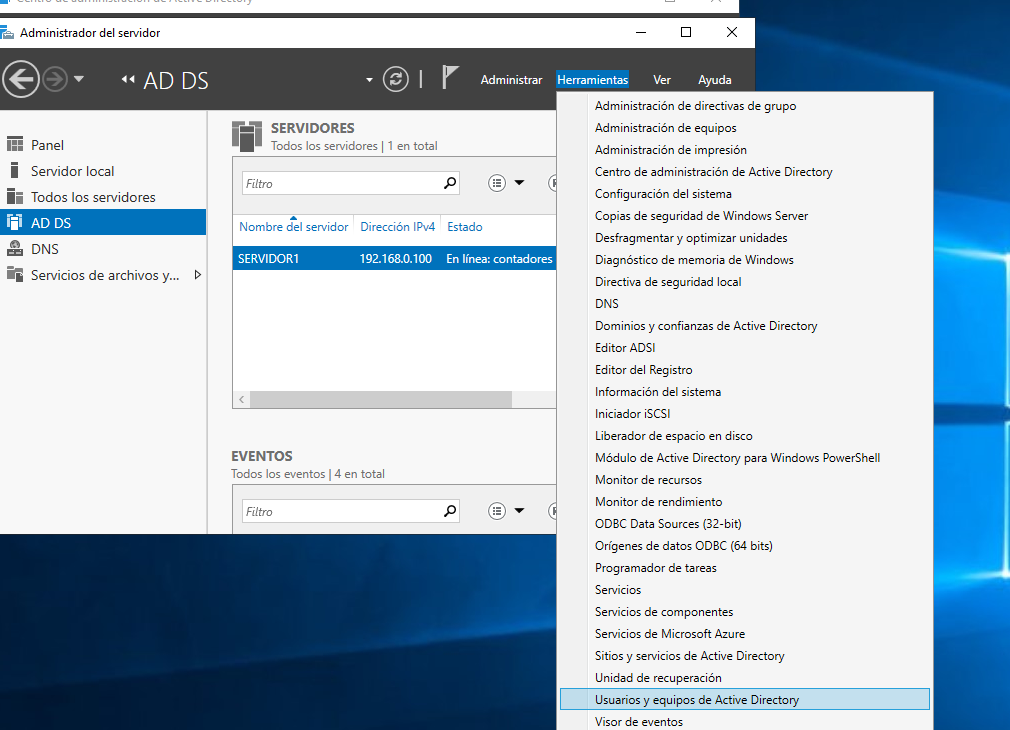
\includegraphics{png/usuaris1.png}

\subsubsection{Creem un usuari}\label{creem-un-usuari}

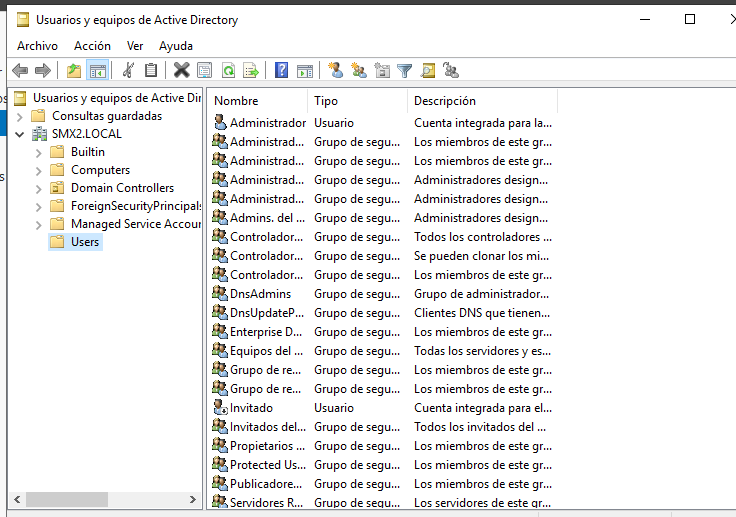
\includegraphics{png/usuaris2.png}

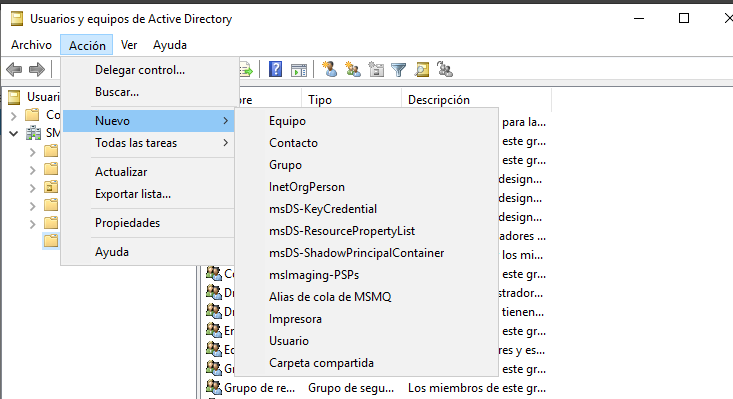
\includegraphics{png/usuaris3.png}

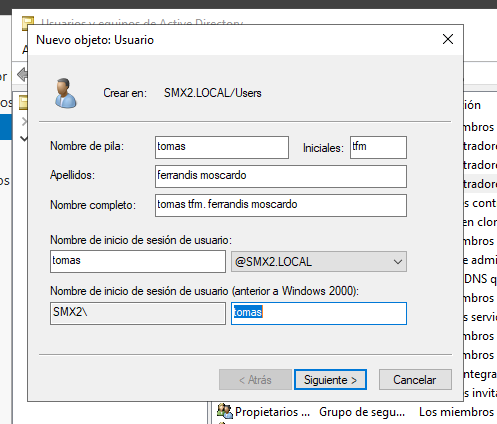
\includegraphics{png/usuaris4.png}

\subsubsection{Configurem el compte d'usuari
creat}\label{configurem-el-compte-dusuari-creat}

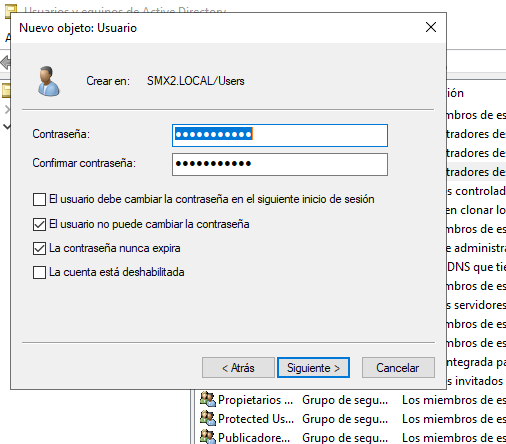
\includegraphics{png/usuaris5.png}

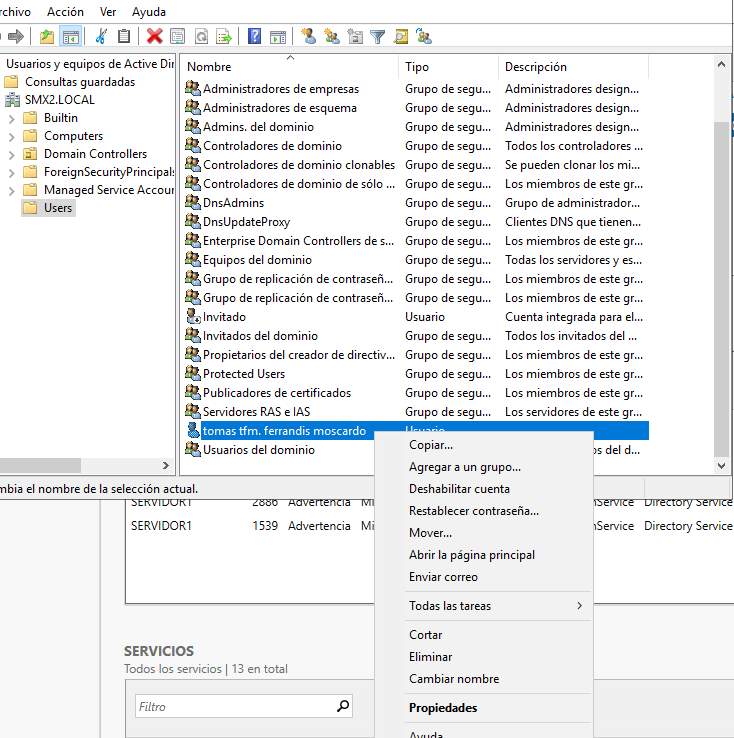
\includegraphics{png/usuaris6.png}

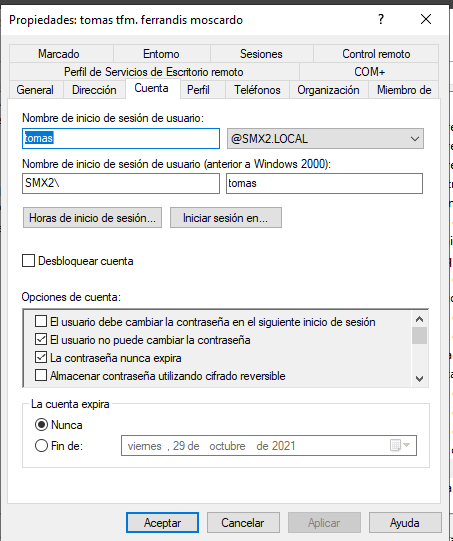
\includegraphics{png/usuaris7.png}

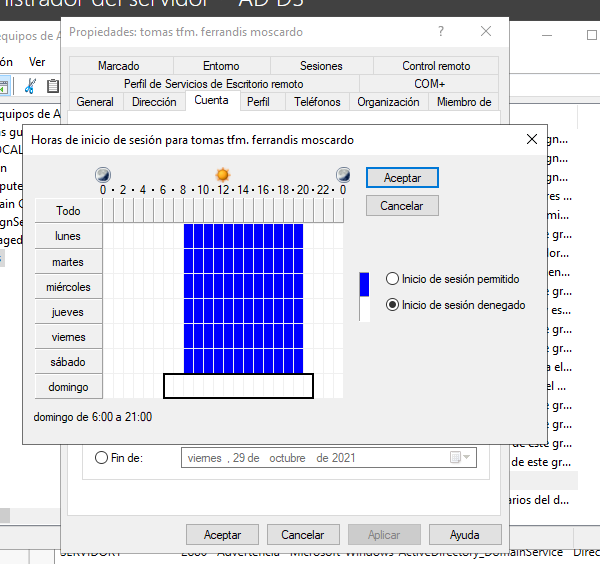
\includegraphics{png/usuaris8.png}

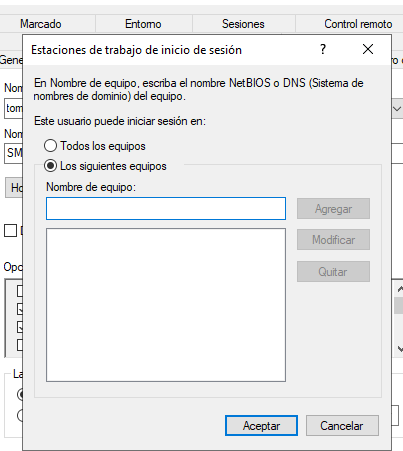
\includegraphics{png/usuaris9.png}

\subsection{4.2 Grups d'usuaris en l'AD}\label{grups-dusuaris-en-lad}

\subsubsection{Tipus i àmbits}\label{tipus-i-uxe0mbits}

Hi ha dos grans tipus de grups al Directori Actiu del Windows:

\textbf{Grups de seguretat:} aquest tipus de grups permet definir
permisos per a recursos del domini. Són els utilitzats a les llistes de
control d'accessos (ACLs) que s'estudiaran més endavant. Aquest tipus de
grups són els que s'utilitzaran a la administració de la xarxa.

\textbf{Grups de distribució:} no tenen característiques de seguretat,
únicament són un llistat d'usuaris per a missatgeria.

Dins dels grups de seguretat hi ha tres àmbits:

\textbf{Grup Universal:} és un grup els permisos del qual s'estenen a
diversos dominis. A més, aquest tipus de grups pot estar format per
usuaris o grups d'usuaris de diferents dominis.

\textbf{Grup Global:} és molt similar als grups universals, és a dir
poden permetre l'accés a recursos de qualsevol dels dominis de l'arbre
del Directori Actiu, però llevat que tots els membres del grup deuen
pertànyer al mateix domini.

\textbf{Grup local del domini:} és un grup creat en un domini amb
membres que poden provenir d'altres dominis i que només pot tenir accés
a recursos dins del domini.

\textbf{En quins casos utilitzarem cada àmbit?}

Els grups universals solen tenir la seva utilitat en grans empreses on
s'ha definit un bosc de dominis assignant dominis a cadascun dels seus
departaments o divisions. En aquest tipus d'estructures, quan se'n
realitza una modificació en el grup, aquesta ha de replicar-se en tots
els controladors de domini que estiguin configurats com a catàleg
global. En xarxes de domini únic es poden aplicar grups globals que
tindran més sentit quan es defineixi un segon domini, el que pot passar
en el moment en què hi hagi una ampliació de l'organització.

Com a pautes generals per a l'administració de xarxes tindrem en compte
les consideracions següents

\begin{enumerate}
\def\labelenumi{\arabic{enumi}.}
\item
  No cal assignar un àmbit més ampli del necessari.
\item
  Els grups locals de domini no es poden processar a altres dominis.
\item
  Un grup global no es replica fora del domini, ja que no forma part del
  pla de replicació del catàleg global.
\item
  Els grups universals es repliquen per tota la xarxa generant trànsit
  que tenia certa incidència en el rendiment abans dels Windows Server
  2008. hui en dia en té poca.
\item
  Si un grup universal està compost per grups globals i es produeixen
  canvis dins dels grups globals, no es produeix un canvi al catàleg
  global, i per tant aquesta modificació no comporta una replicació en
  tots els controladors de domini del bosc.
\end{enumerate}

\subsubsection{Grups predefinits}\label{grups-predefinits}

En instal·lar el Directori Actiu podem comprovar que s'han generat
automàticament una sèrie de grups predefinits amb uns permisos d'acord
amb les funcions assignades:

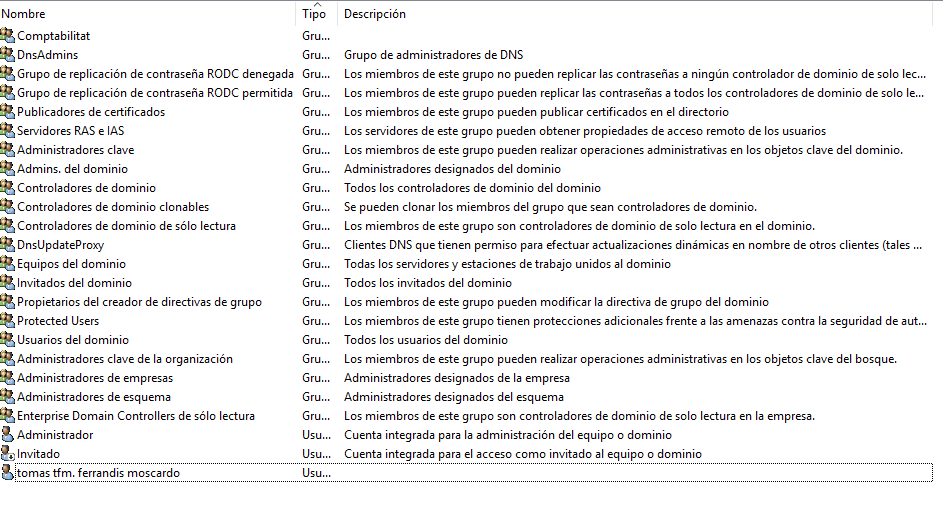
\includegraphics{png/usuaris10.png}

Examinem les funcions d'alguns dels grups més utilitzats:

\textbf{Usuaris del domini:} grup global que conté tots els comptes
d'usuaris del domini.

\textbf{Administradors del domini:} grup global que permet als membres
realitzar tasques d'administració del domini.

\textbf{Administradors d'empresa:} grup universal que permet als membres
realitzar tasques d'administració a tots els dominis de la xarxa.

\textbf{Administradors d'esquema:} grup universal que permet als membres
modificar l'estructura dels objectes del Directori actiu.

\textbf{Administradors:} grup local que permet als seus membres
realitzar tasques d'administració al controlador de domini. Operadors de
còpies de seguretat: grup local que permet als seus membres fer còpies
de seguretat o restaurar fitxers dins del domini.

\textbf{Operadors de compte:} grup local que permet als membres crear,
editar i eliminar comptes d'usuari i grups.

\textbf{Operadors d'impressió:} grup local que permet als membres
configurar i administrar l'ús d'impressores de xarxa.

\textbf{Operadors de servidor:} grup local que permet als seus membres
crear carpetes compartides al servidor i realitzar còpies de seguretat o
restaurar fitxers al controlador de domini.

\textbf{Usuaris:} grup local que limita les possibilitats que un usuari
faci un canvi accidental al sistema però sí permet executar la majoria
de les aplicacions.

\subsection{4.3 Creació de grups.}\label{creaciuxf3-de-grups.}

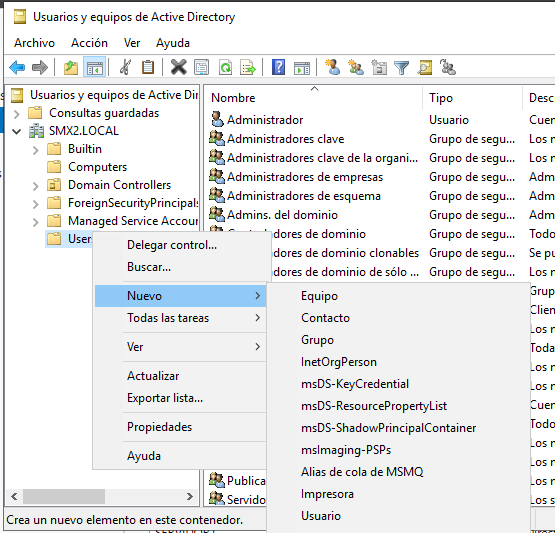
\includegraphics{png/usuaris11.png}

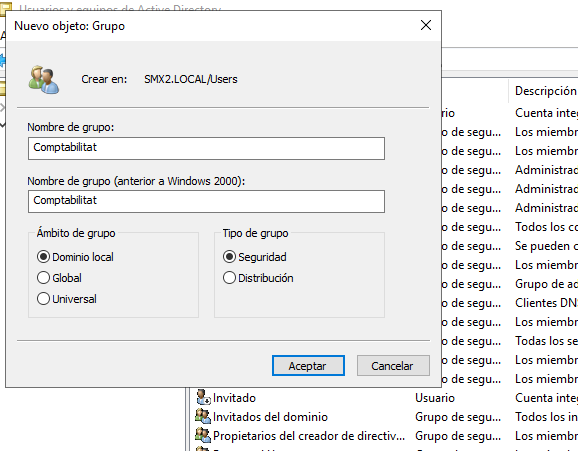
\includegraphics{png/usuaris12.png}

\subsection{4.4 Com afegir usuaris al
grup.}\label{com-afegir-usuaris-al-grup.}

Opció 1: Propietats del grup\ldots{}

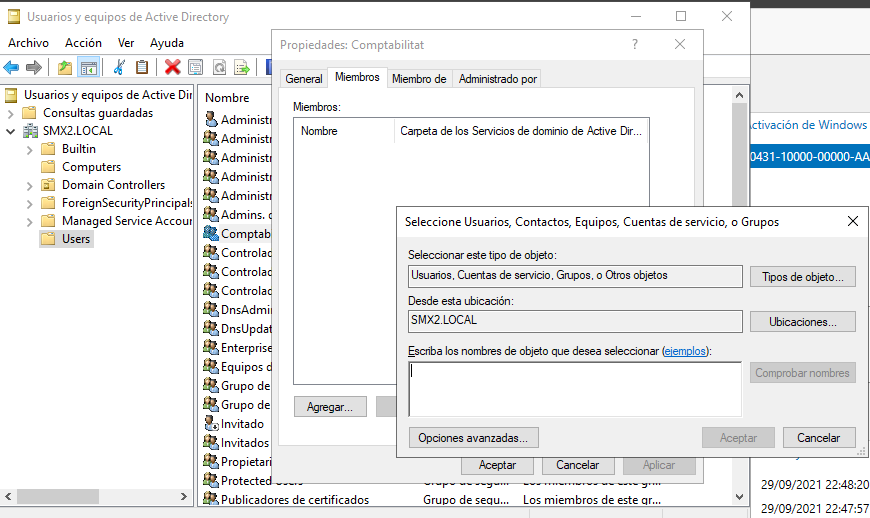
\includegraphics{png/usuaris13.png}

Opció 2: Des de les Propietats de l'usuari\ldots{}

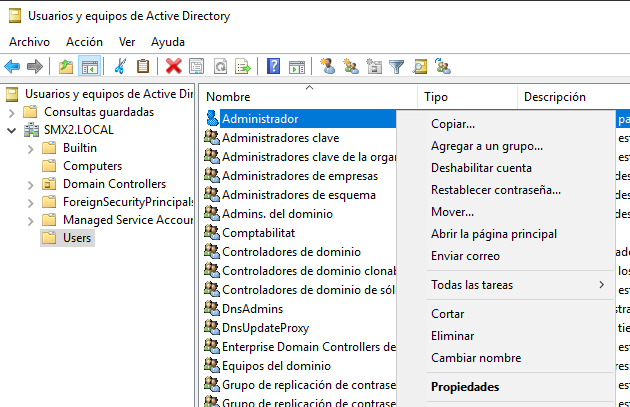
\includegraphics{png/usuaris14.png}

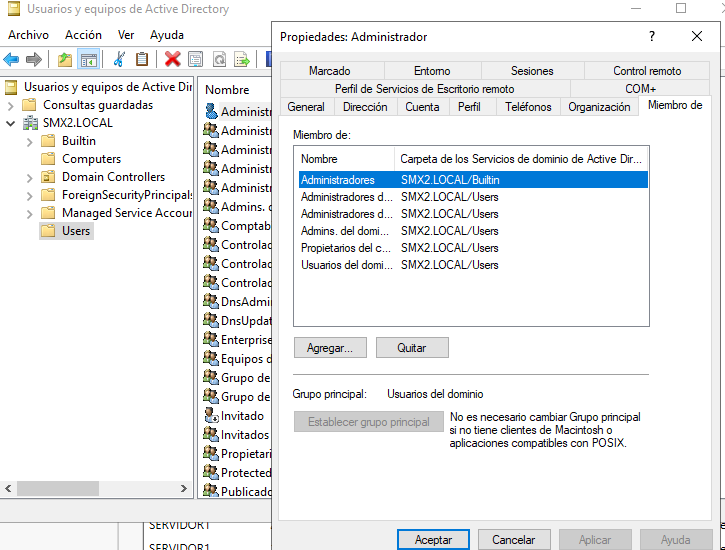
\includegraphics{png/usuaris15.png}

\end{document}
